% id: 82-189
% book: 개념원리 대수 · 08 지수함수의 활용 – 방정식
% section: 연습문제 실력 UP
% figure: crop:fig-82-189.png
% answer: ④
% answer_source: 답지
% variant_level: 0 (원본 전사)
% 이 파일은 build.mjs 가 items.json 에서 만든다. 고칠 때는 items.json 을 고친다.
\smash{\raisebox{4.5mm}{\dmkichul{개념원리 대수 82쪽 189번 · 수능 기출}}}
\noindent\begin{minipage}[t]{0.58\linewidth}\vspace{0pt}\raggedright 직선 $y=2x+k$가 두 함수 $y=\left(\dfrac{2}{3}\right)^{x+3}+1$, $y=\left(\dfrac{2}{3}\right)^{x+1}+\dfrac{8}{3}$의 그래프와 만나는 점을 각각 $\pt{P}$, $\pt{Q}$라 하자. $\seg{PQ}=\sqrt{5}$일 때, 상수 $k$의 값은?\end{minipage}\hfill\begin{minipage}[t]{0.4\linewidth}\vspace{0pt}\centering \setlength{\dmfigw}{120.0pt}\ifdim\dmfigw>\linewidth\setlength{\dmfigw}{\linewidth}\fi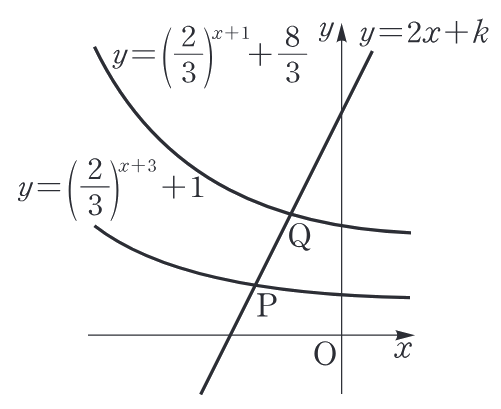
\includegraphics[width=\dmfigw]{figures/fig-82-189.png}\end{minipage}\par
\begin{choices32}{\rule[-3ex]{0pt}{8ex}$\dfrac{31}{6}$}{\rule[-3ex]{0pt}{8ex}$\dfrac{16}{3}$}{\rule[-3ex]{0pt}{8ex}$\dfrac{11}{2}$}{\rule[-3ex]{0pt}{8ex}$\dfrac{17}{3}$}{\rule[-3ex]{0pt}{8ex}$\dfrac{35}{6}$}\end{choices32}
